\documentclass[12pt,a4paper]{article}
%\usepackage{fontspec, xunicode, xltxtra}  
%\setmainfont{Hiragino Sans GB}  
%\usepackage{xeCJK}
%\setCJKmainfont[BoldFont=STZhongsong, ItalicFont=STKaiti]{STSong}
%\setCJKsansfont[BoldFont=STHeiti]{STXihei}
%\setCJKmonofont{STFangsong}

%使用Xelatex编译

% 设置页面
%==================================================
\linespread{2} %行距
% \usepackage[top=1in,bottom=1in,left=1.25in,right=1.25in]{geometry}
% \headsep=2cm
% \textwidth=16cm \textheight=24.2cm
%==================================================

% 其它需要使用的宏包
%==================================================
\usepackage[colorlinks,linkcolor=blue,anchorcolor=red,citecolor=green,urlcolor=blue]{hyperref} 
\usepackage{tabularx}
\usepackage{authblk}         % 作者信息
\usepackage{algorithm}     % 算法排版
\usepackage{amsmath}     % 数学符号与公式
\usepackage{amsfonts}     % 数学符号与字体
\usepackage{mathrsfs}      % 花体
\usepackage{amssymb}
\usepackage[framemethod=TikZ]{mdframed}

\usepackage{graphicx} 
\usepackage{graphics}
\usepackage{color}
\usepackage{xcolor}
\usepackage{tcolorbox}
\usepackage{lipsum}
\usepackage{empheq}

\usepackage{fancyhdr}       % 设置页眉页脚
\usepackage{fancyvrb}       % 抄录环境
\usepackage{float}              % 管理浮动体
\usepackage{geometry}     % 定制页面格式
\usepackage{hyperref}       % 为PDF文档创建超链接
\usepackage{lineno}          % 生成行号
\usepackage{listings}        % 插入程序源代码
\usepackage{multicol}       % 多栏排版
%\usepackage{natbib}         % 管理文献引用
\usepackage{rotating}       % 旋转文字,图形,表格
\usepackage{subfigure}    % 排版子图形
\usepackage{titlesec}       % 改变章节标题格式
\usepackage{moresize}   % 更多字体大小
\usepackage{anysize}
\usepackage{indentfirst}  % 首段缩进
\usepackage{booktabs}   % 使用\multicolumn
\usepackage{multirow}    % 使用\multirow

\usepackage{wrapfig}
\usepackage{titlesec}     % 改变标题样式
\usepackage{enumitem}
\usepackage{aas_macros}

\newcommand{\myvec}[1]%
   {\stackrel{\raisebox{-2pt}[0pt][0pt]{\small$\rightharpoonup$}}{#1}}  %矢量符号
\renewcommand{\vec}[1]{\boldsymbol{#1}}
\newcommand{\me}{\mathrm{e}}
\newcommand{\mi}{\mathrm{i}}
\newcommand{\dif}{\mathrm{d}}
\newcommand{\tabincell}[2]{\begin{tabular}{@{}#1@{}}#2\end{tabular}}

\def\kpc{{\rm kpc}}
\def\km{{\rm km}}
\def\cm{{\rm cm}}
\def\TeV{{\rm TeV}}
\def\GeV{{\rm GeV}}
\def\MeV{{\rm MeV}}
\def\GV{{\rm GV}}
\def\MV{{\rm MV}}
\def\yr{{\rm yr}}
\def\s{{\rm s}}
\def\ns{{\rm ns}}
\def\GHz{{\rm GHz}}
\def\muGs{{\rm \mu Gs}}
\def\arcsec{{\rm arcsec}}
\def\K{{\rm K}}
\def\microK{\mu{\rm K}}
\def\sr{{\rm sr}}
\newcolumntype{p}{D{,}{\pm}{-1}}

\renewcommand{\figurename}{Fig.}
\renewcommand{\tablename}{Tab.}

\renewcommand{\arraystretch}{1.5}

\setlength{\parindent}{0pt}  %取消每段开头的空格

\newcounter{theo}[section]\setcounter{theo}{0}
\renewcommand{\thetheo}{\arabic{section}.\arabic{theo}}
\newenvironment{theo}[2][]{%
\refstepcounter{theo}%
\ifstrempty{#1}%
{\mdfsetup{%
frametitle={%
\tikz[baseline=(current bounding box.east),outer sep=0pt]
\node[anchor=east,rectangle,fill=blue!20]
{\strut Theorem~\thetheo};}}
}%
{\mdfsetup{%
frametitle={%
\tikz[baseline=(current bounding box.east),outer sep=0pt]
\node[anchor=east,rectangle,fill=blue!20]
{\strut Theorem~\thetheo:~#1};}}%
}%
\mdfsetup{innertopmargin=10pt,linecolor=blue!20,%
linewidth=2pt,topline=true,%
frametitleaboveskip=\dimexpr-\ht\strutbox\relax
}
\begin{mdframed}[]\relax%
\label{#2}}{\end{mdframed}}

\newcommand*\widefbox[1]{\fbox{\hspace{2em}#1\hspace{2em}}}


\title{Particle Orbit Theory}
\author{}
\date{\today}
\begin{document}

\maketitle
\cite{1996bspp.book.....B}  Study the motion of charged particles in prescribed electric and magnetic fields.

In a situation where the charged particles do not directly interact with each other and where they do not affect the external magnetic field significantly, the motion of each individual particle can be treated independently. The single particle approach is only valid in \textcolor{red}{very rarified plasmas where collective effects are negligible}. Furthermore, the \textcolor{red}{external magnetic field must be rather strong, much greater than the magnetic field produced by the electric current due to the charged particle motion}.


\section{Motion in a Uniform, Static Magnetic Field}
\cite{2015bps..book.....C} Consider a \textcolor{red}{magnetic field} which is \textcolor{red}{constant in space and time}. The classical equation of motion for a particle of mass $m$ and charge $e_0$ in the field $\vec{B} = (0, 0, B)$ is
\begin{equation}
m\frac{\dif \vec{v}}{\dif t} = m \vec{\ddot{r}} = \frac{e_0}{c} \vec{v} \times \vec{B} ~,
\end{equation}
Since the force on the particle is perpendicular to its velocity,
\begin{equation*}
\ddot{z} = 0 ~,
\end{equation*}
and motion along the field occurs at constant speed, $\dot{z} = v_\parallel$ is constant. Taking the scalar product of the equation of motion with the velocity $\vec{\dot{r}}$:
\begin{equation*}
m\vec{\ddot{r}} \cdot \vec{\dot{r}} = 0 ~,
\end{equation*}
implying that the total kinetic energy energy
\begin{equation*}
\frac{1}{2} m \dot{r}^2 = W = W_\parallel +W_\perp
\end{equation*}
is constant. Since $W_\parallel = \dfrac{1}{2} mv_\parallel^2$ is separately conserved, we find that the kinetic energy of motion perpendicular to the field $W_\perp$ is also constant.

The equation of motion is rewritten in its three cartesian components, 
\begin{eqnarray*}
\frac{\dif v_x}{\dif t} &=& \Omega v_y ~, \\
\frac{\dif v_y}{\dif t} &=& -\Omega v_x ~, \\
\frac{\dif v_z}{\dif t} &=& 0
\end{eqnarray*}
where $\Omega = \dfrac{e_0 B}{mc}$. The solutions are
\begin{eqnarray*}
v_x &=& v_\perp \cos (\Omega t+ \alpha) ~, \\
v_y &=& -v_\perp \sin (\Omega t+ \alpha) ~, \\
v_z &=& v_\parallel ~.
\end{eqnarray*}
The trajectory as a function of time is
\begin{eqnarray*}
x &=& x_0 + \frac{v_\perp}{\Omega} \sin (\Omega t+ \alpha) ~, \\
y &=& y_0 + \frac{v_\perp}{\Omega} \cos (\Omega t+ \alpha) ~, \\
z &=& z_0 +v_\parallel t ~.
\end{eqnarray*}
The trajectory is a helix which positively charged particles sweep in the clockwise sense and negative particles in a counter-clockwise sense as seen projected on the $(x, y)$ plane. The projected orbits are circular with radius \textcolor{red}{$R_L = v_\perp/|\Omega|$}, known as the \textcolor{red}{Larmor radius}. The \textcolor{red}{gyration frequency $|\Omega|$} is known as the \textcolor{red}{cyclotron frequency}, also called the \textcolor{red}{gyrofrequency}.

If define $\vec{\Omega} = \dfrac{e_0\vec{B} }{mc}$,
\begin{equation}
\frac{\dif \vec{v} }{\dif t} = -\vec{\Omega} \times \vec{v} ~,
\end{equation}

\cite{1996bspp.book.....B} The center of the orbit $(x_0, y_0)$ is called the \textcolor{red}{guiding center}. The circular orbit of the charged particle represents a circular current and the direction of the gyration is such that the magnetic field generated by the circular current is opposite to the externally imposed field. It is called \textcolor{red}{diamagnetic effect}.

The \textcolor{red}{pitch angle $\alpha$}, of the helix is defined as
\begin{equation}
\color{red} \alpha = \tan^{-1} \left(\frac{v_\perp}{v_\parallel} \right) ~.
\end{equation}
and depends on the ratio between the perpendicular and parallel velocity components.

The pitch angle of a charged particle is the angle between the particle's velocity vector and the local magnetic field.

\section{Method of Averaging}
\cite{Plasma2014} The motion consists of a rapid oscillation superimposed on a slow secular drift. For such problems, the most efficient approach is to describe the evolution in terms of the average values of the dynamical variables. Consider the equation of motion
\begin{equation}
\dfrac{\dif \vec{z}}{\dif t} = \vec{f}(\vec{z}, t, \tau) ~,
\end{equation}
where $\vec{f}$ is a periodic function of its last argument, with period $2\pi$, and 
\begin{equation}
\tau = t /\epsilon ~.
\label{eq:tau}
\end{equation}
The small parameter $\epsilon$ characterizes the separation between the short oscillation period and the timescale for the slow secular evolution of the ``position" $\vec{z}$.

The basic idea of the averaging method is to treat $t$ and $\tau$ as distinct independent variables, and to look for solutions of the form $\vec{z}(t, \tau)$ that are periodic in $\tau$. Thus, we replace the equation by
\begin{equation}
\dfrac{\partial \vec{z}}{\partial t} +\dfrac{1}{\epsilon} \dfrac{\partial \vec{z}}{\partial \tau}   = \vec{f}(\vec{z}, t, \tau) ~,
\label{eq:z2}
\end{equation}
and reserve Equation (\ref{eq:tau}) for substitution into the final result. The indeterminacy introduced by increasing the number of variables is lifted by the requirement of periodicity in $\tau$. All of the secular drifts are thereby attributed to the variable $t$, while
the oscillations are described entirely by the variable $\tau$.

Let us denote the $\tau$-average of $z$ by $Z$, and seek a change of variables of the form
\begin{equation}
\vec{z}(t, \tau) = \vec{Z}(t) +\epsilon \vec{\zeta}(\vec{Z}, t, \tau) ~.
\end{equation}
$\vec{\zeta}$ is a periodic function of $\tau$ with vanishing mean.
\begin{equation}
\left\langle \vec{\zeta}(\vec{Z}, t, \tau) \right\rangle \equiv \dfrac{1}{2\pi} \oint \vec{\zeta}(\vec{Z}, t, \tau) \dif \tau = 0 ~,
\end{equation}
where $\oint$ denotes the integral over a full period in $\tau$.

The evolution of $\vec{Z}$ is determined by substituting the expansions
\begin{align}
\vec{\zeta} &=  \vec{\zeta}_0(\vec{Z}, t, \tau)  +\epsilon \vec{\zeta}_1(\vec{Z}, t, \tau)  +\epsilon^2 \vec{\zeta}_2(\vec{Z}, t, \tau) + \cdots ~, \\
\dfrac{\dif \vec{Z}}{\dif t} &= \vec{F}_0(\vec{Z}, t)  +\epsilon \vec{F}_1(\vec{Z}, t)  +\epsilon^2 \vec{F}_2(\vec{Z}, t) + \cdots ~, 
\end{align}
into the equation of motion, Equation (\ref{eq:z2}), and solving order by order in $\epsilon$.

To lowest order,
\begin{equation}
\vec{F}_0(\vec{Z}, t) + \dfrac{\partial \vec{\zeta}_0 }{\partial \tau} = \vec{f}(\vec{Z}, t, \tau) ~.
\end{equation}
The solubility condition for this equation is
\begin{equation}
\vec{F}_0(\vec{Z}, t) = \left\langle \vec{f}(\vec{Z}, t, \tau) \right\rangle \equiv \left\langle \vec{f}  \right\rangle(\vec{Z}, t) ~.
\end{equation}
Integrating the oscillating component of Equation yields
\begin{equation}
\vec{\zeta}_0(\vec{Z}, t, \tau) = \int_0^\tau [\vec{f}(\vec{Z}, t, \tau^\prime) - \left\langle \vec{f}  \right\rangle(\vec{Z}, t)] \dif \tau^\prime ~.
\end{equation}
To first order,
\begin{equation}
\vec{F}_1 +\dfrac{\partial \vec{\zeta}_0 }{\partial t}  +\vec{F}_0 \cdot \nabla \vec{\zeta}_0 + \dfrac{\partial \vec{\zeta}_1 }{\partial \tau} =  \vec{\zeta}_0 \cdot \nabla \vec{f}(\vec{Z}, t, \tau) ~.
\end{equation}
The solubility condition for this equation yields
\begin{equation}
\vec{F}_1(\vec{Z}, t) = \left\langle \vec{\zeta}_0 (\vec{Z}, t, \tau) \cdot \nabla\vec{f}(\vec{Z}, t, \tau)  \right\rangle \equiv \left\langle \vec{\zeta}_0 \cdot \nabla\vec{f} \right\rangle (\vec{Z}, t) ~.
\end{equation}
The final result is
\begin{equation}
\dfrac{\dif \vec{Z}}{\dif t}  = \left\langle \vec{f}  \right\rangle(\vec{Z}, t) + \epsilon \left\langle \vec{\zeta}_0 \cdot \nabla\vec{f} \right\rangle (\vec{Z}, t) + \mathcal O (\epsilon^2) ~.
\end{equation}
The secular motion of the ``guiding center" position $\vec{Z}$ is determined to lowest order by the average of the ``force" $\vec{f}$, and to next order by the correlation between the oscillation in the ``position" $\vec{z}$ and the oscillation in the spatial gradient of the ``force".

\section{Guiding Center Motion}
\cite{Plasma2014} Consider the motion of a charged particle of mass $m$ and charge $e$ in the limit in which the electromagnetic fields experienced by the particle do not vary much in a gyroperiod, so that
\begin{align}
& \rho |\nabla \vec{B}| \ll B ~, \\
& \dfrac{1}{\Omega} \dfrac{\partial B}{\partial t}  \ll B ~.
\end{align}



\section{Motion in Orthogonal Electric and Magnetic Fields}
\cite{1996bspp.book.....B} Taking the electric field into consideration will result in a drift of the particle superimposed onto its gyratory motion. The exact nature of this \textcolor{red}{electric drift} depends on whether the field is electrostatic or time-varying and whether it is spatially uniform or not.

Consider an electrostatic field, $\vec{E}$, which can have both the perpendicular components and the component parallel to $\vec{B}$ separately. The parallel component
\begin{equation}
m \dot{v}_\parallel = q E_\parallel ~,
\end{equation}
describes a straightforward acceleration along the magnetic field. However, in geophysical plasmas most parallel electric fields cannot be sustained, since they are immediately canceled out by electrons, which are under most circumstances extremely mobile along the magnetic field lines.

\cite{2015bps..book.....C} Assume a \textcolor{red}{constant, homogeneous electric field $\vec{E}$ orthogonal to $\vec{B}$}:
\begin{eqnarray*}
\vec{E} &=& \color{red} (0, E, 0) ~,\\
\vec{B} &=& (0, 0, B)
\end{eqnarray*}
with $E$ and $B$ independent of position and time. The $y$ component of the equation of motion is
\begin{equation*}
\frac{\dif v_y}{\dif t} = -\Omega v_x + \frac{e_0 E}{m} = -\Omega \left(v_x -\frac{Ec}{B} \right)
\end{equation*}
Consider a frame of reference \textcolor{cyan}{$S^\prime$}, \textcolor{cyan}{moving at the speed $\dfrac{Ec}{B}$ along the $x$ direction}, which is possible as long as \textcolor{orange}{$E \ll B$}: in this case the Lorentz transformation reduces to the Galilean transformation
\begin{eqnarray*}
x^\prime &=& x -\frac{Ect}{B} ~, \\
y^\prime &=& y ~,\\
z^\prime &=& z ~, \\
t^\prime &=& t ~,
\end{eqnarray*}
and in the frame $S^\prime$ the equation of motion along $y^\prime$ becomes
\begin{equation}
\frac{\dif v^\prime_y}{\dif t} = -\Omega v^\prime_x 
\end{equation}
In the \textcolor{cyan}{original frame of reference}, the \textcolor{cyan}{trajectory is a superposition of the original helical trajectory} and \textcolor{purple}{a uniform translation at speed $\dfrac{Ec}{B}$ along the $x$-axis}. 

\cite{1996bspp.book.....B} An ion is accelerated into the direction of the electric field, thereby increasing its gyroradius. But it is decelerated during the second half of its gyratory orbit, now with decreasing gyroradius. The different gyroradii shift the position of the guiding center in the $\vec{E} \times \vec{B}$ direction. The electrons are accelerated when moving antiparallel to the electric field and decelerated when moving parallel. But since their sense of gyration is opposite, too, their guiding centers drift into the same direction.

%===========================================================================================================================
\begin{figure*}
\centering
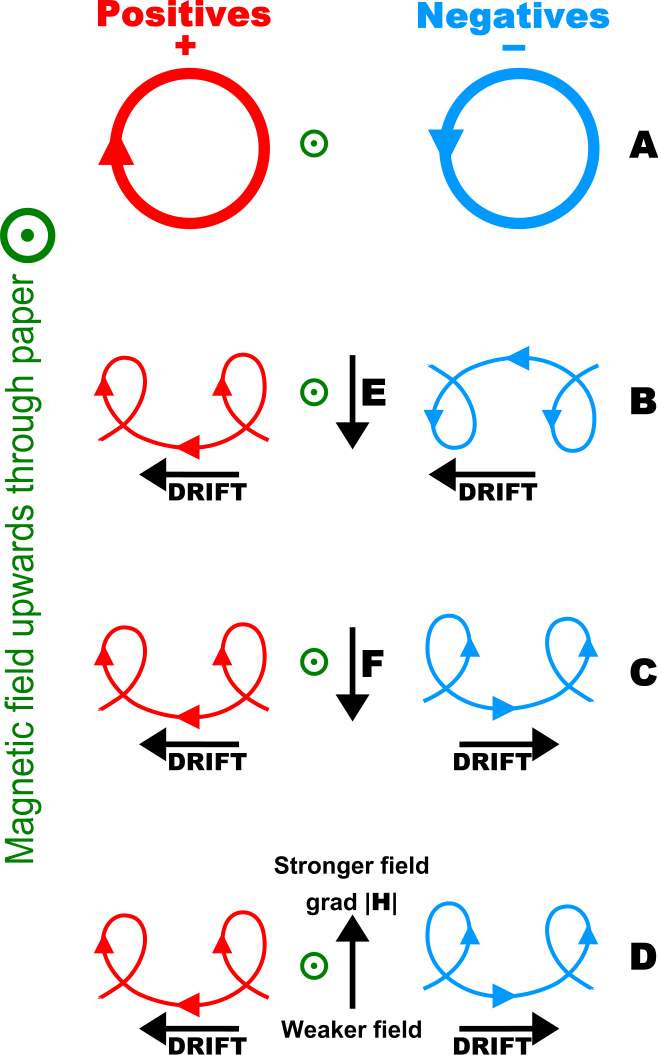
\includegraphics[height=12.cm, angle=0]{Charged-particle-drifts.png}
\caption{Charged particle drifts in a homogeneous magnetic field. (A) No disturbing force; (B) With an electric field, $E$; (C) With an independent force, $F$ (e.g. gravity); (D) In an inhomogeneous magnetic field, grad $H$.
}
\label{fig:cpd}
\end{figure*}
%===========================================================================================================================


\cite{2015bps..book.....C} Consider that the effect of the electric field in the $y$-direction is to accelerate (or decelerate, depending on the charge) a particle along that axis. In the presence of a magnetic field, the \textcolor{yellow}{increase (decrease) in speed along that direction leads to an increasing (decreasing) centripetal force deflecting the motion orthogonally to both $\vec{E}$ and $\vec{B}$. This force gradually changes the direction of motion eventually leading to a change of sign of $v_y$, so that motion in the $y$-direction is confined to a finite displacement}. On the other hand the \textcolor{red}{different radius of curvature of the gyrating motion as the particle moves along and against the direction of the electric field leads to the average uniform displacement orthogonal to the fields}. The velocity is known as the \textcolor{red}{drift velocity $\vec{v}_E$} and may be written in a coordinate independent way as
\begin{equation}
\vec{v}_E = c\frac{\vec{E} \times \vec{B}}{B^2} ~.
\end{equation}
\begin{empheq}[box=\widefbox]{align*}
& m \dfrac{\dif \vec{v}}{\dif t} = q (\vec{E} +\vec{v} \times \vec{B}) \\
& m \dfrac{\dif \vec{v} \times \vec{B} }{\dif t} = q \vec{E} \times \vec{B} + q(\vec{v} \times \vec{B}) \times \vec{B} \\
& m \dfrac{\dif \vec{v} \times \vec{B} }{\dif t} = q \vec{E} \times \vec{B} -q(B^2 \vec{v} -(\vec{v}\cdot \vec{B})\vec{B}) \\
& \dfrac{\dif \vec{v}_\perp \times \vec{\hat{B}} }{\dif t} = \dfrac{qB}{m} \left[ -\vec{v}_{\perp} +\dfrac{\vec{E}\times \vec{B}}{B^2}\right]
\end{empheq}

\cite{1996bspp.book.....B} The $\vec{E} \times \vec{B}$ drift has a fundamental physical root in the Lorentz transformation of the electric field into the moving system of the particle. In this system the electric field is given by
\begin{equation}
\vec{E}^\prime = \vec{E} + \vec{v} \times \vec{B} ~.
\end{equation}
For a free particle this field must vanish, $\vec{E}^\prime = 0$, which yields for the electric field
\begin{eqnarray}
\vec{E} = -\vec{v} \times \vec{B} ~.
\end{eqnarray}
Solving for the velocity immediately yields the expression for the electric drift
\begin{equation}
\vec{v}_E = \dfrac{\vec{E} \times \vec{B}}{B^2} ~.
\end{equation}
Take the cross-product of both sides with $\vec{B}$, 
\begin{eqnarray*}
\vec{E} \times \vec{B} &=&  -(\vec{v} \times \vec{B}) \times \vec{B} \\
&=& \vec{B}\times (\vec{v} \times \vec{B}) \\
&=& B^2 \vec{v} -(\vec{v} \cdot \vec{B})\vec{B} \\
&=& B^2 \vec{v}_\perp
\end{eqnarray*}
which is
\begin{equation}
\vec{v}_\perp = \frac{\vec{E} \times \vec{B}}{B^2} 
\end{equation}
Because the Lorentz transformation does not depend on the charge of the particles, the $\vec{E}\times \vec{B}$ drift is also independent of the sign of the charge.

\cite{2015bps..book.....C} When \textcolor{cyan}{$E/B = O(1)$}, \textcolor{purple}{relativistic corrections} become important, and a different approach is required if $E > B$, since $v_x$ in this case would become:
\begin{equation*}
v_x = c\frac{E}{B} +v_{0x} \cos (\Omega t) ~,
\end{equation*}
which exceeds the speed of light. With $E > B$, use the relativistic equations of motion,
\begin{eqnarray*}
\frac{\dif \vec{p}}{\dif t} &=& e_0(\vec{E} +\frac{\vec{v}}{c} \times \vec{B}) ~,\\
\vec{p} &=& \gamma m \vec{v} ~, \\
\gamma &=& \frac{1}{\sqrt{1-v^2/c^2}} ~.
\end{eqnarray*}
Consider the Lorentz transformation along the positive $x$-axis with speed $v$ on electric and magnetic fields:
\begin{align} 
E^\prime_x &= E_x ~, & B^\prime_x &= B_x ~,\\
E^\prime_y &= \gamma(E_y -\beta B_z) ~, & B^\prime_y &= \gamma (B_y +\beta E_z) ~,\\
E^\prime_z &= \gamma(E_z +\beta B_y) ~, & B^\prime_z &= \gamma (B_z -\beta E_y) ~,
\end{align} 
where $\beta = v/c$. Then $E^\prime_x = 0, E^\prime_z = 0$, \textcolor{blue}{$E^\prime_y = \gamma(E - \beta B)$}. For \textcolor{cyan}{$E < B$}, the choice \textcolor{cyan}{$\beta = \dfrac{E}{B}$ makes the $y$ component of the electric field in the $S^\prime$ frame vanish}, and only a magnetic field along $z^\prime  = z$, \textcolor{blue}{$B^\prime_z$} $= \gamma (B -\beta E) = \gamma(B - E^2/B)=$ \textcolor{blue}{$B/\gamma$} will remain, yielding the helical motion. In the original frame $S$ the motion is a superposition of the helical motion and the translational one.

Which kind of Lorentz transformation used to simplify the equations of motion may be understood by recalling the two Lorentz invariants for the electromagnetic field, \textcolor{red}{$\vec{E}\cdot  \vec{B}$} and \textcolor{red}{$E^2 - B^2$}. If the first of these vanishes, it will \textcolor{red}{always be possible to find a frame in which either $E$ or $B$ vanishes, depending on the sign of the second invariant $E^2 - B^2$}. If the electric and magnetic fields are perpendicular, but \textcolor{purple}{$E > B$}, \textcolor{purple}{a new frame can be found with a vanishing magnetic field}, corresponding to a Lorentz boost along the $x$ direction with \textcolor{cyan}{$\beta = \dfrac{B}{E}$}. Once the equation of motion is solved in the new frame, one can transform the solution back to the original frame applying the inverse Lorentz transformation with $\beta = -B/E$ along the $x^\prime$ axis.

The \textcolor{purple}{drift speed $\vec{v}_E$ does not depend on the sign of the charge of the particle} in motion. Both electrons and protons move with the same speed under this drift, and \textcolor{orange}{no current is generated} by the so called \textcolor{red}{``$\vec{E} \times \vec{B}$" drift} within the plasma. 


When there is any \textcolor{orange}{constant force $\vec{F}$ orthogonal to the magnetic field $\vec{B}$}: it will give rise to a \textcolor{orange}{drift which is orthogonal both to the force and the magnetic field}, whose magnitude is 
\begin{equation}
\color{red} \vec{v}_F = c \frac{\vec{F} \times \vec{B}}{e_0 B^2} ~,
\end{equation}
The \textcolor{orange}{drift from a non-electric force will give rise to an average current in the plasma}. \fbox{%  
This drift depends on the charge.}  


The case \textcolor{red}{$E = B$} is related to the motion of a particle in the field of an electromagnetic wave and the method of a Lorentz boost, used to treat the cases with $E \neq B$, is no longer applicable. We have to solve directly the equation of motion of special relativity in the laboratory frame. Consider a particle of mass $m$ and charge $e_0$, initially at rest at the origin of the coordinates, acted upon by a linearly polarized electromagnetic wave of frequency $\omega$.  Choose a frame of reference in which the electric field lies on the $x$-axis and the magnetic field on the $y$-axis, then the waves propagates along the $z$-direction. 
\begin{eqnarray*}
\vec{E} = E_0 \cos \phi ~\vec{e}_x ~,\\
\vec{B} = E_0 \cos \phi ~\vec{e}_y ~,
\end{eqnarray*}
with $\phi = \omega (t-z/c)$. The equations of relativistic dynamics are
\begin{eqnarray*}
\frac{\dif (m\gamma \vec{v})}{\dif t} &=& e_0 (\vec{E} +\vec{\beta} \times \vec{B}) ~, \\
\frac{\dif (m\gamma c)}{\dif t} &=& e_0 \vec{E} \cdot \vec{\beta} ~.
\end{eqnarray*}
Introduce \textcolor{blue}{$\omega_E = (e_0 E_0/mc)$},
\begin{eqnarray*}
\frac{\dif (\gamma \beta_x)}{\dif t} &=& \omega_E (1-\beta_z) \cos \phi ~, \\
\frac{\dif (\gamma \beta_y)}{\dif t}  &=& 0 ~, \\
\frac{\dif (\gamma \beta_z)}{\dif t}  &=& \omega_E \beta_x \cos \phi ~, \\
\frac{\dif \gamma}{\dif t}  &=& \omega_E \beta_x \cos \phi ~,
\end{eqnarray*}
so
\begin{equation}
\frac{\dif \gamma(1-\beta_z)}{\dif t}  = 0 ~,
\end{equation}
\textcolor{red}{$\gamma(1-\beta_z) = K$  is a constant of motion}.
To determine the trajectory of particle, using $\phi$ in place of $t$,
\begin{equation*}
\vec{\beta} = \frac{1}{c} \frac{\dif \vec{r}}{\dif t} = \frac{1}{c} \frac{\dif \vec{r}}{\dif \phi}  \frac{\dif \phi}{\dif t} = \frac{\omega}{c} (1-\beta_z) \frac{\dif \vec{r}}{\dif \phi} = \frac{\omega}{c} (1-\beta_z) \vec{r}^\prime ~.
\end{equation*}
The prime indicates the derivative with respect to $\phi$. And
\begin{equation*}
\frac{\dif (\gamma \vec{\beta})}{\dif t} = \frac{\dif}{\dif t} \left[\gamma \frac{\omega}{c} (1-\beta_z) \vec{r}^\prime \right] =  \frac{\omega^2 K}{c} (1-\beta_z) \vec{r}^{\prime\prime} ~.
\end{equation*}

\begin{eqnarray*}
x^{\prime\prime} &=& \frac{c}{\omega K} \frac{\omega_E}{\omega} \cos \phi ~, \\
y^{\prime\prime} &=& 0 ~, \\
z^{\prime\prime} &=& \frac{1}{K} \frac{\omega_E}{\omega} x^{\prime} \cos \phi ~.
\end{eqnarray*}
Since $\vec{r}(0) = 0$ and $\vec{\dot{r}}(0) = 0$ (the dot indicates the time-derivative), 
\begin{eqnarray*}
\phi(0) = 0 ~, ~~\dot{\phi}(0) = \omega [1-\beta_z(0)] = \omega ~, ~~ K = K(0) = 1~,
\end{eqnarray*}
and the initial conditions for the system above are:
\begin{eqnarray*}
x(0) = 0 ~, ~~x^\prime(0) = \dot{x}(0)/\dot{\phi}(0) = 0 ~, ~~ y(0) = y^\prime(0) = 0 ~, ~~ z(0) = z^\prime(0) = 0
\end{eqnarray*}
The second equation shows that $y = 0$: no motion occurs in the $y$-direction. A straightforward integration of the other two equations gives
\begin{eqnarray*}
x &=& -\frac{\omega_E}{\omega} \frac{c}{\omega} (1-\cos \phi) ~, \\
z &=& \left( \frac{\omega_E}{2\omega} \right)^2 \frac{c}{\omega} (\phi -\frac{1}{2}\sin 2\phi) = \xi(\phi -\frac{1}{2} \sin 2\phi) ~,
\end{eqnarray*}
with
\begin{equation*}
\xi = \left( \frac{\omega_E}{2\omega} \right)^2 \frac{c}{\omega} ~.
\end{equation*}

\begin{equation*}
z = \omega \xi(t-\frac{z}{c}) -\frac{\xi}{2} \sin 2\phi
\end{equation*}
or
\begin{equation}
z = \left(\frac{\omega \xi}{1+\omega \xi/c} \right) t -\left(\frac{\xi}{2(1+\omega \xi/c)} \right) \sin 2\phi ~~~\fbox{%  
$\phi$ is a function of $z$ and $t$.}
\end{equation}
The \textcolor{cyan}{velocity along $z$} is a  \textcolor{orange}{superposition of a constant speed plus a periodic term}. The constant term corresponds to a value of $\beta_z$, 
\begin{equation*}
\beta_z = \frac{\omega \xi/c}{1+\omega \xi/c} = \frac{(\omega_E/2\omega)^2}{1+(\omega_E/2\omega)^2} ~,
\end{equation*}
When \textcolor{red}{$(\omega_E /\omega)$ is very large}, namely when \textcolor{red}{$E_0$ is very large or $\omega$ is very small}, it tends to unity. The first circumstance arises in the field of an \textcolor{violet}{intense laser beam} or in \textcolor{violet}{linear accelerators}. The second one has been considered in connection with the problem of the  \textcolor{violet}{acceleration of cosmic rays in the vicinity of a pulsar}. The pulsar emits a low frequency electromagnetic wave, which in principle could accelerate particles to very large energies. This model, however, presents a number of drawbacks and has been abandoned. 

The periodic term, coupled with the motion along $x$, produces an \textcolor{cyan}{eight-shaped trajectory in the $(x,z)$ plane of a frame moving along $z$ with a speed $c\beta_z$}.


\subsection{Polarization Drift}
\cite{1996bspp.book.....B}
\begin{equation}
m\frac{\dif \vec{v}}{\dif t} = q(\vec{E} +\vec{v} \times \vec{B}) ~,
\end{equation}
Take the cross-product of both sides with $\dfrac{\vec{B} }{B^2}$
\begin{eqnarray*}
\frac{m}{q}\frac{\dif \vec{v}}{\dif t} \times \frac{\vec{B} }{B^2} &=& \frac{(\vec{E} +\vec{v} \times \vec{B}) \times \vec{B} }{B^2}  \\
&=& \frac{\vec{E} \times \vec{B} }{B^2} + \frac{(\vec{v} \times \vec{B}) \times\vec{B} }{B^2} \\
&=& \frac{\vec{E} \times \vec{B} }{B^2} -\frac{ B^2 \vec{v} -(\vec{v} \cdot \vec{B})  \vec{B} }{B^2} \\
\end{eqnarray*}
\begin{eqnarray*}
\vec{v} -\frac{ \vec{B}(\vec{v} \cdot \vec{B}) }{B^2} = \frac{\vec{E} \times \vec{B} }{B^2} -\frac{m}{q}\frac{\dif \vec{v}}{\dif t} \times \frac{\vec{B} }{B^2}
\end{eqnarray*}
The left-hand side is a perpendicular velocity vector and the first term on the right-hand side is the $\vec{E} \times \vec{B}$ drift. \textcolor{yellow}{Averaging over the gyroperiod and thus neglecting temporal changes of the order of the gyroperiod or faster} allows to \textcolor{yellow}{take the perpendicular velocity as the perpendicular drift velocity, $\vec{v}_d$}. The magnetic field is assumed time independent,
\begin{equation}
\vec{v}_d = \vec{v}_E - \frac{m}{qB^2} \frac{\dif (\vec{v} \times \vec{B}) }{\dif t} = \vec{v}_E +\frac{1}{\omega_g B} \frac{\dif E_\perp}{\dif t}
\end{equation}
 where $\omega_g = \dfrac{qB}{m}$, and $\vec{E}_\perp = -\vec{v} \times \vec{B}$. It describes the \textcolor{red}{drift of a charged particle in crossed homogeneous magnetic and electric fields, where the electric field is allowed to vary slowly}. The last term in equation is called \textcolor{red}{polarization drift},
\begin{equation}
\color{red} \vec{v}_P = \frac{1}{\omega_g B} \frac{\dif \vec{E}_\perp}{\dif t}
\end{equation}
There is an important qualitative difference between the polarization drift and the $\vec{E} \times \vec{B}$ drift. The $\vec{E} \times \vec{B}$ drift does neither depend on the charge nor on the mass of the particle, since it can be viewed as a result of the Lorentz transformation. Thus electrons, protons, and heavier ions all \textcolor{red}{move into the same direction perpendicular to $\vec{B}$ and $\vec{E}$ with the same velocity}. The polarization drift, on the other hand, \textcolor{red}{increases proportional to the mass of the particle}. It is \textcolor{red}{directed along the electric field}, but \textcolor{red}{oppositely for electrons and ions}. It creates a current
\begin{equation}
\vec{j}_P = e n_e (\vec{v}_{Pi} -\vec{v}_{Pe}) = \frac{n_e(m_i +m_e)}{B^2} \dfrac{\dif \vec{E}_\perp}{\dif t}
\end{equation}
which carries electrons and ions into opposite directions and polarizes the plasma. Since $m_i > m_e$, the \textcolor{purple}{polarization current is mainly carried by the ions}.

\subsection{Electric Drift Correction}
\cite{1996bspp.book.....B} Equation
\begin{equation*}
\vec{v}_d = \vec{v}_E - \frac{m}{qB^2} \frac{\dif (\vec{v} \times \vec{B}) }{\dif t} = \vec{v}_E +\frac{1}{\omega_g B} \frac{\dif E_\perp}{\dif t}
\end{equation*}
can also describe the drift due to \textcolor{orange}{inhomogeneities of the electric field} if the total time derivative is taken as the sum of the temporal and the convective derivative $\dif /\dif t = \partial /\partial t +\vec{v} \cdot \nabla$, where the velocity vector can, to a good approximation, be replaced by the $\vec{E} \times \vec{B}$ velocity. The convective term becomes proportional to $E^2$. It is a nonlinear contribution and is usually much smaller than the time derivative and therefore neglected in most cases.

The convective derivative takes into account spatial variations of the electric field in the direction of the $\vec{E} \times \vec{B}$ drift under the assumption that the \textcolor{blue}{electric field changes only gradually}. When this is not the case and the \textcolor{blue}{electric field changes considerably over one gyroradius}, there is a further \textcolor{blue}{correction on the electric field drift}, known as \textcolor{red}{finite Larmor radius effect}. This correction is a \textcolor{green}{second order effect in $r_g$} and leads to the more complete expression for the electric field drift
\begin{equation}
\color{yellow} \vec{v}_E = (1 +\frac{r_g^2 \nabla^2}{4} ) \frac{\vec{E} \times \vec{B} }{B^2} 
\end{equation}
where $r_g$ is the gyroradius,
\begin{equation}
r_g = \dfrac{v_\perp}{\Omega_g} = \dfrac{mv_\perp}{|q| B} ~.
\end{equation}
The second spatial derivative takes account of the \textcolor{red}{spatial variation of the electric field, averaged over the gyration orbit}. Finite Larmor radius effects are normally neglected in macroscopic applications of particle motion but may become \textcolor{cyan}{important in the vicinity of plasma boundaries}, \textcolor{cyan}{plasma transitions} and \textcolor{cyan}{small scale structures} in a plasma.


\section{Motion in Slowly Variable Magnetic Fields}
\cite{2015bps..book.....C} Because \textcolor{cyan}{the electric and magnetic fields in space are never uniform or constant in time}, there are in general \textcolor{cyan}{no exact integrals of motion} to which one can resort to simplify the understanding of charged particle dynamics. When particle \textcolor{cyan}{motion occurs in slowly variable magnetic fields, either in time or in space}, the equation of particle motion may be solved approximately. The systematic \textcolor{red}{expansion in terms of drift velocities of higher order} is allowed if the the \textcolor{red}{ratio of the Larmor radius $R_L$ to the gradient scale $L$}, \textcolor{red}{$R_L/L \ll 1$}, or alternatively, if the \textcolor{red}{characteristic frequency of time variation of the field $1/T$ is much smaller than the gyrofrequency $|\Omega|$}, i.e. \textcolor{red}{$|\Omega|T \gg1$}. When these conditions are satisfied, exact integrals of motion are replaced by \textcolor{red}{approximate integrals} or \textcolor{red}{adiabatic invariants}, whose relative changes are bounded by inequalities more stringent than the ones above.

\cite{1996bspp.book.....B} A typical magnetic field has gradients and often field lines are curved. This inhomogeneity of the magnetic field leads to a \textcolor{blue}{magnetic drift} of charged particles. Time variations of the magnetic field itself cannot impart energy to a particle, since the Lorentz force is always perpendicular to the velocity of the particle. However, since $\partial \vec{B}/\partial t = -\nabla \times \vec{E}$, the associated inhomogeneous electric field may accelerate the particles. 

\subsection{Charged Particle Orbits in the Presence of a Magnetic Fields with a Weak Gradient}
\cite{2015bps..book.....C} Equation 
\begin{equation*}
\vec{v}_F = c \frac{\vec{F} \times \vec{B}}{e_0 B^2} ~,
\end{equation*}
can be used to understand particle motion by use of a local analysis in a magnetic field with gradients. Consider \textcolor{cyan}{a magnetic field line having a certain curvature}. The particle will locally gyrate around the magnetic field, which may be considered constant on the scale of the Larmor radius. The particle generally also has a motion parallel to the field $\vec{B}$, and, because of the \textcolor{yellow}{curvature of the field line}, the \textcolor{yellow}{particle will feel in its own frame of reference an outward centrifugal force due to this motion $\vec{F} = (mv_\parallel^2 \vec{R}_c)/R_c^2$}, where \textcolor{cyan}{$R_c$ is the local radius of curvature}. As a consequence of curvature, a drift motion will arise with velocity
\begin{equation}
\color{red} \vec{v}_C = \frac{mc v_\parallel^2 (\vec{R}_c \times \vec{B})}{e_0 R_c^2 B^2} = \frac{2c W_\parallel}{e_0 R_c B} (\hat{\vec{R}}_c \times \hat{\vec{B}}) ~,
\end{equation}
\textcolor{cyan}{$\hat{\vec{B}}$ is the unit vector tangent to the local magnetic field}, and \textcolor{cyan}{$\hat{\vec{R}}_c$ the unit vector along the radius of curvature}. The factor in parentheses is a purely geometrical term which describes the \textcolor{red}{local geometry of magnetic field lines}. This motion of charged particles is called the \textcolor{red}{curvature drift}.

Consider a magnetic field directed along one direction, whose \textcolor{cyan}{magnitude depends on a coordinate along an axis orthogonal to the magnetic field $\vec{B}$} itself. Assume $\vec{B} = [0, 0, B(y)]$, where $B(y)$ satisfies the \textcolor{cyan}{weak gradient condition}
\begin{equation*}
\frac{\dif B/\dif y}{B} R_L \ll 1 ~.
\end{equation*}
The Lorentz force around a given point $y_0$ is
\begin{equation*}
F(y) = F(y_0 +\delta_y) = \frac{e_0}{c} [B (-v_x \vec{e}_y +v_y \vec{e}_x)]_{y_0+\delta y} ~,
\end{equation*}
which only shows the motions in a plane perpendicular to the magnetic field $\vec{B}$.

Denoting $y$-derivatives with a prime, the field in the neighborhood of this point may be written as $B(y_0 + \delta y) = B(y_0) + \delta y B^\prime(y_0) = B_0 + \delta y B_0^\prime$,
\begin{equation}
\vec{F}(y) = \frac{e_0 B_0}{c} \left[-v_x \vec{e}_y +v_y \vec{e}_x \right] +\frac{e_0 B_0}{c} \left[-v_x \vec{e}_y +v_y \vec{e}_x \right] \delta y \frac{B_0^\prime}{B_0} ~.
\end{equation}
For $\delta y$ is of the same order as $R_L$, $\delta y \dfrac{B_0^\prime}{B_0} \ll 1$. The first term in the equation describes the unperturbed circular motion while the second term provides the first order correction. We can thus \textcolor{yellow}{assume that $v_x,  v_y,  \delta y = y -y_0$ are the same as those obtained from the motion in a constant magnetic field, which are periodic functions of the phase $\phi = \Omega t + \alpha$}. Averaging the force $\vec{F}$ over a gyration period, $P = 2\pi/|\Omega|$, 
\begin{equation*}
\langle \vec{F} \rangle = \frac{1}{P} \int_0^P \vec{F} \dif t ~,
\end{equation*}
in which the only non zero contribution comes from the term $v_x \delta y B_0^\prime$. 
\begin{equation*}
\langle \vec{F} \rangle = -\frac{e_0 B^\prime_0}{cP} \int_0^P v_x \delta y \dif t \vec{e}_y = -\frac{e_0 v_\perp R_L B^\prime_0}{cP} \int_0^P \cos^2 \phi \dif t \vec{e}_y = -\frac{e_0 v_\perp R_L B^\prime_0}{2c}  \vec{e}_y = -\frac{1}{2} mv^2_\perp \frac{B_0^\prime}{B_0} \vec{e}_y ~.
\end{equation*}
\textcolor{red}{On averaging over a gyroperiod}, there is a \textcolor{red}{constant force perpendicular to $\vec{B}_0$}, which gives rise to a \textcolor{red}{drift orthogonal to both $\vec{B}_0$ and $\langle \vec{F} \rangle$}. The drift velocity is
\begin{equation*}
\vec{v}_G = {\color{red} - ?} \frac{cW_\perp B^\prime_0}{e_0 B^2_0} \vec{e}_x ~,
\end{equation*}
 whose general vector expression is
 \begin{equation}
\color{red} \vec{v}_G = \frac{cW_\perp (\vec{B}_0 \times \nabla) |\vec{B}_0|}{e_0 |B_0|^3} ~,
\end{equation}
known as the \textcolor{red}{gradient drift}.

When the gradients are small with respect to the cyclotron radius and the fastest time-scale is given by the gyro-motion. One calls the averaged position of the particle over one gyroperiod the guiding center of the particle. The particle executes a gyromotion around its guiding center while the guiding center itself moves following the drifts in question. In order for the so-called guiding center approximation to be valid, an additional condition must be established concerning the parallel motion: the distance a particle moves along the field during one gyroperiod must also be small respect to the scale of gradients, or \textcolor{red}{$v_\parallel P \ll L$}.

The equations of motion along and across the magnetic field are
\begin{eqnarray}
\nonumber m\frac{\dif \vec{v}_\parallel}{\dif t} &=& \vec{F}_\parallel \\
m\frac{\dif \vec{v}_\perp}{\dif t} &=& \vec{F}_\perp +\frac{e_0}{c} (\vec{v}_\perp \times \vec{B}) ~.
\end{eqnarray}
Write $\vec{v}_\perp = \vec{v}_\Omega + \vec{v}_d$, where $\vec{v}_\Omega$ is the velocity of the cyclotron motion around the guiding center and orthogonal to the local magnetic field while $\vec{v}_d$ is the drift velocity. Now expand
\begin{equation*}
\vec{v}_d = \vec{v}^0_d +\vec{v}^1_d +\vec{v}^2_d +\cdots 
\end{equation*}
and expand the equations for the drifts order by order in the small gradient parameter:
\begin{equation}
m\left(\frac{\dif \vec{v}^0_d}{\dif t} + \cdots\right) = \frac{e_0}{c} (\vec{v}^1_d +\cdots ) \times \vec{B} ~,
\end{equation}
considering that the \textcolor{cyan}{time-dependence of the zero-order drift is a small quantity},
\begin{equation*}
\vec{v}^1_d = -\frac{mc}{e_0 B} \left(\frac{\dif \vec{v}^0_d}{\dif t} \times \frac{\vec{B}}{B} \right)
\end{equation*}
and so on and so forth. Generally the first order drift may differ in direction from the zero order drift, and must therefore be included to understand charged particle trajectories.

\cite{1996bspp.book.....B} The inhomogeneity of the magnetic field leads to a magnetic drift of charged particles. Time variations of the magnetic field itself cannot impart energy to a particle, since the Lorentz force is always perpendicular to the velocity of the particle. However, since $\partial \vec{B}/\partial t = -\nabla \times \vec{E}$, the associated inhomogeneous electric field may accelerate the particles.

\subsection{Gradient Drift}
\cite{1996bspp.book.....B} Assume that the magnetic field is \textcolor{blue}{weakly inhomogeneous}, for example increasing in the upward direction. The gyroradius of a particle decreases in the upward direction and thus the gyroradius of a particle will be larger at the bottom of the orbit than at the top half. As a result, \textcolor{red}{ions and electrons drift into opposite directions, perpendicular to both $\vec{B}$ and $\nabla B$}.

Assume that the \textcolor{blue}{typical scale length of a magnetic field gradient is much larger than the particle gyroradius}, we can Taylor expand the magnetic field vector about the guiding center of the particle
\begin{equation}
\vec{B} = \vec{B}_0 +(\vec{r}\cdot \nabla) \vec{B}_0 ~,
\end{equation}
where $\vec{B}_0$ is measured at the guiding center and $\vec{r}$ is the distance from the guiding center. 
\begin{equation}
m \dfrac{\dif \vec{v}}{\dif t} = q(\vec{v} \times \vec{B}_0) +q[\vec{v} \times (\vec{r}\cdot \nabla) \vec{B}_0] ~,
\end{equation}
Expanding the velocity term into a gyration and a drift motion, $\vec{v} = \vec{v}_g +\vec{v}_\nabla$, and noting $v_\nabla \ll v_g$, 
\begin{equation}
m \dfrac{\dif \vec{v}_\nabla}{\dif t} = q(\vec{v}_\nabla \times \vec{B}_0) +q(\vec{v}_g \times (\vec{r} \cdot \nabla)\vec{B}_0) ~,
\end{equation}
where we have omitted the terms describing gyration in a homogeneous field and neglected $\vec{v}_\nabla \times  (\vec{r}\cdot \nabla) \vec{B}_0$ as a small quantity.

Since we are interested in \textcolor{red}{time scales much larger than the gyroperiod}, we can \textcolor{red}{average over one gyration}. Upon this the left side vanishes since \textcolor{yellow}{any acceleration a particle experiences when moving into the weak field region is balanced by a deceleration when moving into the strong field region in the other half of its gyratory orbit}. Since we know that $\vec{v}_\nabla$ lies in the plane perpendicular to the magnetic field, take the cross-product with $\vec{B}_0/B_0^2$. 
\begin{equation}
\vec{v}_\nabla = \dfrac{1}{B^2_0} \langle (\vec{v}_g \times (\vec{r} \cdot \nabla) \vec{B}_0) \times \vec{B}_0 \rangle
\end{equation}
where the angle brackets denote \textcolor{red}{averaging over one gyroperiod}. Assuming $\vec{B}$ to vary only in the $x$ direction, $\vec{B}_0 = B_0(x) \vec{\hat{e}}_z$,
\begin{equation}
\vec{v}_\nabla = -\dfrac{1}{B_0} \left\langle \vec{v}_g x \dfrac{\dif B_0}{\dif x} \right\rangle
\end{equation}
Replace $\vec{v}_g$ and $x$ by 
\begin{align}
& \nonumber x-x_0 = r_g \sin \omega_g t \\
& \nonumber y-y_0 = r_g \cos \omega_g t ~,
\end{align}
\begin{align}
& v_{\nabla x} = -\dfrac{v_\perp r_g}{B_0} \left\langle \sin \omega_g t \cos \omega_g t \dfrac{\dif B_0}{\dif x} \right\rangle \\
& v_{\nabla y} = \dfrac{v_\perp r_g}{B_0} \left\langle \sin^2 \omega_g t \dfrac{\dif B_0}{\dif x} \right\rangle ~,
\end{align}
Taking the \textcolor{yellow}{gyroperiod average, $v_{\nabla x}$ will vanish} since it contains the product of sine and cosine terms. Averaging over the $\sin^2$ term yields a factor $1/2$. Thus the drift will have \textcolor{red}{only a $y$ component}
\begin{equation}
\vec{v}_{\nabla} = \pm \dfrac{v_\perp r_g}{2 B_0} \dfrac{\partial B_0}{\partial x} \vec{\hat{e}}_y ~,
\end{equation}
where the direction of the motion depends on the sign of the charge. Since the direction of the magnetic field gradient was chosen arbitrarily, this can be generalized
\begin{equation}
\color{red} \vec{v}_{\nabla} = \dfrac{m v_\perp^2}{2 q B^3} (\vec{B} \times \nabla B) ~,
\end{equation}
showing that a \textcolor{blue}{magnetic field gradient} leads to a \textcolor{red}{gradient drift} \textcolor{blue}{perpendicular to both the magnetic field and its gradient}. It shows that \textcolor{red}{ions and electrons drift into opposite directions} and that, furthermore, the gradient drift velocity is  \textcolor{red}{proportional to the perpendicular energy of the particle}, $W_\perp = \dfrac{1}{2}mv_\perp^2$. \textcolor{violet}{More energetic particles drift faster, since they have a larger gyroradius and experience more of the inhomogeneity of the field}.

As in the case of the \textcolor{yellow}{polarization drift}, the opposite drift directions of electrons and ions lead to a \textcolor{red}{transverse current}. This \textcolor{red}{gradient drift current} has the form
\begin{equation}
\color{red} \vec{j}_\nabla = n_e e(\vec{v}_{\nabla i} -\vec{v}_{\nabla e}) = \dfrac{n_e(\mu_i +\mu_e)}{B^2} \vec{B} \times \nabla B ~,
\end{equation}
where the \textcolor{red}{magnetic moment}
\begin{equation}
\color{red} \mu = \dfrac{m v_\perp^2}{2B} = \dfrac{W_\perp}{B} ~,
\end{equation}
to describe the \textcolor{red}{ratio between perpendicular particle energy and magnetic field}.

\subsection{General Force Drift}
\cite{1996bspp.book.....B} A more general form of \textcolor{yellow}{guiding center drift}, which is valid not only for the Coulomb force, but for any force acting on a charged particle in a magnetic field is
\begin{equation}
\color{red} \vec{v}_F = \dfrac{1}{\omega_g} \left (\dfrac{\vec{F}}{m} \times \dfrac{\vec{B}}{B} \right) ~,
\end{equation}
\textcolor{red}{All particle drifts} can be described this way by using the appropriate force terms, whenever the \textcolor{red}{drift velocity of the particle is much smaller than its gyrovelocity}. For the gradient, the polarization, and the gravitational drift, these forces can be written as
\begin{align}
& \color{red} \vec{F}_\nabla = -\mu \nabla B ~,\\
& \color{red} \vec{F}_P = -m \dfrac{\dif \vec{E}}{\dif t} ~, \\
& \color{red} \vec{F}_G = -m\vec{g} ~,
\end{align}
where $\vec{F}_\nabla$ denotes the gradient and $\vec{F}_P$ the polarization force. $\vec{F}_G$ is the gravitational force, which is typically much weaker than the other forces. Except for processes near the solar surface, it can usually be neglected.

It shows  \textcolor{red}{all drifts generated by a force other than the Coulomb force depend on the sign of the charge}, since $\omega_g$ carries this sign. Hence, for these drifts ions and electrons run into opposite directions, creating a transverse current. Moreover, these  \textcolor{red}{drifts depend on the mass of the charge carriers} and thus the  \textcolor{red}{drift velocities are typically quite different for ions and electrons}.

\subsection{Curvature Drift}
\cite{1996bspp.book.....B} The gradient drift is only one component of the particle drift in an inhomogeneous magnetic field. When the field lines are curved, a curvature drift appears. Due to their parallel velocity, $v_\parallel$, the particles experience a centrifugal force
\begin{equation}
\vec{F}_R = m v_\parallel^2 \dfrac{\vec{R}_c}{R_c^2} ~,
\end{equation}
where $\vec{R}_c$, is the local radius of curvature. The curvature drift is
\begin{equation}
\vec{v}_R = \dfrac{m v_\parallel^2}{q} \dfrac{\vec{R}_c \times \vec{B}}{R_c^2 B^2} ~.
\end{equation}
The curvature drift is proportional to the parallel particle energy, $W_\parallel = \dfrac{1}{2} mv_\parallel^2$,and perpendicular to the magnetic field and its curvature. It creates a transverse current since ion and electron drifts have opposite signs. The curvature drift current has the form
\begin{equation}
\vec{j}_R = n_e e (\vec{v}_{R i} - \vec{v}_{Re}) = \dfrac{2n_e (W_{i \parallel} +W_{e\parallel})}{R_c^2 B^2} (\vec{R}_c \times \vec{B}) ~,
\end{equation}
As the associated drift, the curvature current flows perpendicular to both the curvature of the magnetic field and the magnetic field itself.

In a cylindrically symmetric field, it turns out that $-\nabla B = (B/R_c^2)\vec{R}_c$. Add the gradient to the curvature drift to obtain the total magnetic drift
\begin{equation}
\vec{v}_B = \vec{v}_R +\vec{v}_\nabla = (v_\parallel^2 +\dfrac{1}{2} v_\perp^2) \dfrac{\vec{B} \times \nabla B}{\omega_g B^2}
\end{equation}
It is the transverse current associated with this full magnetic drift which creates the magnetospheric ring current.


\section{Adiabatic Invariants}
\cite{Plasma2014} Poincar\'e invariants are generally of little practical interest unless the curve $C$ closely corresponds to the trajectories of actual particles. An \textcolor{red}{approximate Poincar\'e invariant} may thus be obtained by choosing the curve $C$ to be \textcolor{red}{a circle of points corresponding to a gyrophase period}.
\begin{equation}
\mathcal I \simeq I = \oint \vec{p} \cdot \dfrac{\partial \vec{q}}{\partial \gamma} \dif \gamma ~.
\end{equation}
$I$ is an adiabatic invariant. 

To evaluate $I$ for a magnetized plasma, recall that the canonical momentum for charged particles is
\begin{equation}
\vec{p} = m \vec{v} + e \vec{A} ~,
\end{equation}
where $\vec{A}$ is the vector potential. Let us express $\vec{A}$ in terms of its Taylor series about the guiding center position:
\begin{equation}
\vec{A}(\vec{r}) = \vec{A}(\vec{R}) +(\vec{\rho}\cdot \nabla) \vec{A}(\vec{R}) +\mathcal O(\rho^2) ~.
\end{equation}
The element of length along the curve $C(t)$ is
\begin{equation}
\color{yellow} \dif \vec{r} = \dfrac{\partial \vec{\rho}}{\partial \gamma} \dif \gamma = \dfrac{\vec{u}}{\Omega} \dif \gamma ~.
\end{equation}
The adiabatic invariant is
\begin{align}
\nonumber  I &= \color{yellow}  \oint \dfrac{\vec{u}}{\Omega} \cdot (m[\vec{U} +\vec{u}] +e[\vec{A} +(\vec{\rho}\cdot \nabla) \vec{A}]) \dif \gamma +\mathcal O(\epsilon) ~, \\
&= \color{yellow}  2\pi m \dfrac{u_\perp^2}{\Omega} + 2\pi \dfrac{e}{\Omega} \left\langle \vec{u} \cdot (\vec{\rho}\cdot \nabla) \vec{A} \right\rangle +\mathcal O(\epsilon) ~.
\end{align}
The final term on the right-hand side is written
\begin{equation}
\color{yellow}  2\pi e \left\langle (\vec{\rho}\times\vec{b})  \cdot (\vec{\rho}\cdot \nabla) \vec{A} \right\rangle = -2\pi e \dfrac{u_\perp^2}{2 \Omega^2} \vec{b} \cdot \nabla \times \vec{A} = -\pi m \dfrac{u_\perp^2}{\Omega} ~.
\end{equation}
It follows that
\begin{equation}
I = 2\pi \dfrac{m}{e} + \mathcal O(\epsilon) ~.
\end{equation}
Thus, to lowest order, the adiabatic invariant is proportional to the magnetic moment, $\mu$. 



\cite{1996bspp.book.....B} Adiabatic invariants are not absolute constants like total energy or total momentum, but may change both in space and time. There essence is, however, that they \textcolor{red}{change very slowly compared with some typical periodicities of the particle motion}.

For particles in electromagnetic fields, adiabatic invariants are associated with each type of motion the particle can perform. The \textcolor{red}{magnetic moment, $\mu$}, is associated with the \textcolor{blue}{gyration about the magnetic field}, the \textcolor{red}{longitudinal invariant, $J$}, with the \textcolor{blue}{longitudinal motion along the magnetic field}, and the third invariant, \textcolor{red}{$\Phi$}, with the \textcolor{blue}{perpendicular drift}. 

Whenever these \textcolor{green}{motions are periodic} and \textcolor{green}{changes in the system have angular frequencies much smaller than the oscillation frequency of the particle corresponding to one of the above motions}, the \textcolor{orange}{action integral}
\begin{equation}
\color{orange} J_i = \oint p_i \dif q_i ~,
\end{equation}
is a \textcolor{orange}{constant of the motion} and describes an adiabatic invariant. The pair of variables $(p_i ,q_i)$ are the generalized momentum and coordinate of Hamiltonian mechanics, and the integration has to be done over  \textcolor{blue}{one full cycle of $q_i$}.

\subsection{Magnetic Moment Conservation}
\cite{2015bps..book.....C} Consider a magnetic field with \textcolor{cyan}{cylindrical symmetry} in which the magnetic field has a \textcolor{cyan}{strong axial component} and  satisfies the conditions for \textcolor{cyan}{weak gradients}. The field can be written in cylindrical coordinates $r, \theta, z$ as
\begin{equation*}
\vec{B} = [B_r(r,z), 0, B_z(r,z)] ; ~\textcolor{red}{B_z \gg B_r} ~\rightarrow ~ B = (B_r^2 +B_z^2)^{1/2} \simeq B_z ~.
\end{equation*}
From the divergence free condition for the magnetic field $\nabla \cdot B = 0$,
\begin{equation*}
\frac{1}{r} \frac{\partial}{\partial r}(r B_r) +\frac{\partial B_z}{\partial z} = 0 ~,
\end{equation*}
which may be integrated
\begin{equation*}
\int_0^r \frac{\partial (r B_r)}{\partial r} \dif r = -\int_0^r r \frac{\partial B_z}{\partial z} \dif r \simeq -\left\langle \frac{\partial B}{\partial z} \right\rangle \frac{r^2}{2} ~.
\end{equation*}
where $r$ is considered to be of the same order as the Larmor radius $R_L$ and that the magnetic field and the magnetic field gradients vary on a much larger scale. 

\begin{equation*}
B_r \simeq -\frac{r}{2} \left\langle \frac{\partial B}{\partial z} \right\rangle ~,
\end{equation*}
The equation of motion of a particle in the direction parallel to the magnetic field is
\begin{equation*}
m \frac{\dif v_\parallel}{\dif t} = -\frac{e_0}{c} (\vec{v} \times \vec{B})_z = -\frac{e_0}{c} v_\theta B_r ~. \color{red} ?
\end{equation*}
The sense of particle gyration is opposite in sign to the charge, we may write
\begin{equation*}
v_\theta = -\frac{e_0}{|e_0|} v_\perp ~, \color{red} ?
\end{equation*}
therefore
\begin{equation*}
\frac{\dif v_\parallel}{\dif t} = -\frac{e_0}{c} \left( -\frac{e_0}{|e_0|} v_\perp \right) \left(-\frac{r}{2} \frac{\partial B}{\partial z} \right) \simeq -\left(\frac{|e_0|}{c} R_L |\Omega| \frac{R_L}{2} \right) \frac{\partial B}{\partial z} = -\left(\frac{|e_0| \pi R_L^2}{cP} \right) \frac{\partial B}{\partial z} 
\end{equation*}
where the gyroperiod is $P = 2\pi/|\Omega|$.

The periodic gyromotion of a charged particle $e_0$ in the plane orthogonal to the magnetic field is electrically equivalent to a current carrying loop with $I = |e_0|/P$. According to Amp\`ere's law, such a loop corresponds to a magnetic dipole with \textcolor{red}{magnetic moment $\mu$},
\begin{eqnarray*}
\mu = \frac{IS}{c} &=& \frac{|e_0|}{c} \frac{\pi R_L^2}{P} \\
&=& \frac{\pi |e_0|}{cP} \left(\frac{mv_\perp c}{e_0 B}\right)^2 \\
&=& \frac{2\pi}{P} \left(\equiv \Omega = \frac{|e_0| B}{mc} \right) \frac{m^2 v^2_\perp c}{2|e_0| B^2} \\
&=& \frac{mv_\perp^2}{2B} = \frac{W_\perp}{B}
\end{eqnarray*}
Therefore along $\vec{B}$,
\begin{equation*}
m \frac{\dif v_\parallel}{\dif t} = -\mu \frac{\partial B}{\partial z} ~,
\end{equation*}
multiplying by $v_\parallel$ leads to
\begin{equation*}
\frac{\dif W_\parallel}{\dif t} = m v_\parallel\frac{\dif v_\parallel}{\dif t} = -\mu v_\parallel \frac{\partial B}{\partial z} = -\mu \frac{\dif B}{\dif t} ~,
\end{equation*}
where we have used
\begin{equation*}
\frac{\dif }{\dif t} = \frac{\partial }{\partial t} +\vec{v} \cdot \nabla ~.
\end{equation*}
Since the magnetic field does no work on the particles and there is no explicit time-dependence of the field itself, the total energy of the particle is conserved :
\begin{equation*}
\frac{\dif W (= W_\perp +W_\parallel)}{\dif t} = 0\Longrightarrow \frac{\dif W_\perp}{\dif t} = -\frac{\dif W_\parallel}{\dif t} = \mu \frac{\dif B}{\dif t} ~,
\end{equation*}
The time-derivative of $\mu$ is
\begin{equation*}
\frac{\dif \mu}{\dif t} = \frac{\dif }{\dif t} \left( \frac{W_\perp}{B} \right) = \frac{1}{B} \frac{\dif W_\perp}{\dif t} -\frac{W_\perp}{B^2} \frac{\dif B}{\dif t} = \frac{\mu}{B} \frac{\dif B}{\dif t} -\frac{\mu B}{B^2} \frac{\dif B}{\dif t} = 0 ~.
\end{equation*}
The \textcolor{purple}{magnetic moment is a conserved quantity}, i.e. an \textcolor{red}{adiabatic invariant}, provided \textcolor{orange}{gradient lengthscales of the average field are small compared to the particle gyro-radii}. In the particle's frame of reference, the magnetic field changes, albeit slowly with time, because of the motion of the particle.

Consider a \textcolor{blue}{slowly varying field}, directed along the axis in a cylindrical coordinate system: $B = [0, 0, B(t)]$, whose typical time variation $T$ is much longer than the gyroperiod $2\pi/|\Omega|$. The time-variation induces an azimuthal electric field $\vec{E}$ which appears in the perpendicular components of the equation of motion. Taking the scalar product of the equation of motion with $\vec{v}_\perp$,
\begin{equation*}
m\frac{\dif \vec{v}_\perp}{\dif t} \cdot \vec{v}_\perp = e_0 \vec{E} \cdot \vec{v}_\perp ~,
\end{equation*}
or
\begin{equation*}
\frac{\dif \left(\dfrac{1}{2} mv_\perp^2 \right)}{\dif t} = e_0 \vec{E} \cdot \vec{v}_\perp ~.
\end{equation*}
Integrating this over the gyroperiod, from time $0$ to $P = 2\pi/|\Omega|$, the left hand side gives the variation of the kinetic energy of perpendicular motion over one gyroperiod $W_\perp$:
\begin{equation*}
\Delta W_\perp = e_0 \int_0^P \vec{E} \cdot \vec{v}_\perp \dif t = e_0 \oint \vec{E} \cdot \dif \vec{r}_\perp = e_0 \int_S (\nabla \times \vec{E}) \cdot \dif \vec{S} ~,
\end{equation*}
where $\dif \vec{r}_\perp = \vec{v}_\perp \dif t$ while $\dif S$ is an oriented element of the surface upon which the cyclotron motion orbit rests.

\begin{equation}
\Delta W_\perp = - \frac{e_0}{c}  \int_S \frac{\partial \vec{B}}{\partial t} \cdot \dif \vec{S} \simeq \frac{\pi R_L^2 |e_0| \dot{B} }{c} ~,
\end{equation}
where $\left\langle \dfrac{\partial B}{\partial t} \right\rangle = \dot{B}$ is assumed because of slow variations of the magnetic field. We have taken into account the sign coming from the orientation of particle orbits of different sign.

Since $R_L = |\vec{v}_\perp|/|\Omega|$,
\begin{equation*}
\Delta W_\perp = W_\perp \frac{2\pi}{|\Omega|} \frac{\dot{B}}{B} ~.
\end{equation*}
$\dfrac{2\pi \dot{B}}{|\Omega|}$ is the change of $B$ over a gyroperiod, i.e. $\Delta B$,
\begin{eqnarray*}
\Delta W_\perp = W_\perp \frac{\Delta B}{B} ~,
\end{eqnarray*}
\begin{eqnarray*}
\boxed{ \frac{\Delta W_\perp}{B} = W_\perp \frac{\Delta B}{B^2} ~, \Longrightarrow \frac{\Delta W_\perp}{B} - W_\perp \frac{\Delta B}{B^2} = 0 ~, \Longrightarrow} \Delta (W_\perp/B) = \Delta(\mu) = 0 ~,
\end{eqnarray*}
The \textcolor{red}{magnetic moment is an adiabatic invariant in the slowly time-varying magnetic fields}

\cite{1996bspp.book.....B} The magnetic moment of a particle does not change when the particle moves into stronger or weaker magnetic fields. Consider the energy conservation equation
\begin{equation}
W = W_\parallel +W_\perp ~.
\end{equation}
Since $W$ is a constant in the absence of electric fields, its time derivative vanishes
\begin{equation}
\dfrac{\dif W_\parallel}{\dif t} + \dfrac{\dif W_\perp}{\dif t} = 0 ~.
\end{equation}
For the transverse energy, $W_\perp = \mu B$, 
\begin{equation}
 \dfrac{\dif W_\perp}{\dif t} = \mu  \dfrac{\dif B}{\dif t} +B  \dfrac{\dif \mu}{\dif t} ~.
\end{equation}
$\dif B/\dif t = v_\parallel \dif B/\dif s$ is the \textcolor{blue}{variation of the magnetic field as seen by the particle along its guiding center trajectory}. The magnetic field itself is assumed to be constant. The parallel particle energy can be derived from the parallel component of the gradient force which gives the parallel equation of motion
\begin{equation}
m \dfrac{\dif v_\parallel}{\dif t} = -\mu \nabla_\parallel B = -\mu \dfrac{\dif B}{\dif s}
\end{equation}
Multiplying the left-hand side of equation with $v_\parallel$ and the right-hand side with its equivalent, $\dif s /\dif t$, one finds for the time derivative of the parallel energy
\begin{equation}
\dfrac{\dif W_\parallel}{\dif t} = -\mu \dfrac{\dif B}{\dif t} ~.
\end{equation}
\begin{equation}
\dfrac{\dif W_\parallel}{\dif t} + \dfrac{\dif W_\perp}{\dif t} = B  \dfrac{\dif \mu}{\dif t} = 0 ~,
\end{equation}
which yields that the magnetic moment is an invariant of the particle motion. The \textcolor{red}{magnetic moment is not affected by small changes in the cyclotron frequency or the gyroradius which occur when the magnetic field changes along the particle path}.

Up to now we have neglected electric fields, which can accelerate particles. Thus we have neglected temporal changes of the magnetic field, since $\partial \vec{B}/\partial t = -\nabla \times \vec{E}$. However, \textcolor{red}{when the magnetic field fluctuations are slow enough, the magnetic moment is still conserved}. Consider the change in perpendicular particle energy caused by an electric field, 
\begin{equation}
\dfrac{\dif W_\perp}{\dif t} = q(\vec{E} \cdot \vec{v}_\perp) ~.
\end{equation}
The gain in energy over one gyration is obtained by integrating over the gyroperiod
\begin{equation}
\Delta  W_\perp = q \int_0^{2\pi/\omega_g} (\vec{E} \cdot \vec{v}_\perp)  \dif t ~.
\end{equation}
If the field changes slowly, the particle orbit is closed and we can replace the time integral by a line integral over the unperturbed orbit. Using Stokes' theorem
\begin{equation}
\Delta  W_\perp = q \oint_C \vec{E} \cdot \dif \vec{s} = q \int_A (\nabla \times \vec{E}) \cdot \dif \vec{A}  = -q \int_A \dfrac{\partial \vec{B}}{\partial t} \cdot \dif \vec{A} 
\end{equation}
where $\dif \vec{s} = \vec{t} \dif s$ is the product of a line element, $\dif s$, of the closed gyratory orbit, $C$, with the line element's tangent vector, $\vec{t}$, and $\dif \vec{A} = \vec{n} \dif A$ is the product of a surface element, $\dif A$ of the plane, $\vec{A}$, enclosed by the orbit and the surface element's normal vector, $\vec{n}$. For  \textcolor{red}{changes in the field much slower than the gyroperiod}, $\partial \vec{B}/\partial t$ can be replaced by $\omega_g \Delta B/2\pi$, with $\Delta B$ the average change during one gyroperiod
\begin{equation}
\Delta  W_\perp = \dfrac{1}{2} q \omega_g r^2_g \Delta B = \mu \Delta B ~.
\end{equation}
The change in perpendicular energy is given by
\begin{equation}
\Delta  W_\perp = \mu \Delta B + B \Delta \mu
\end{equation}
and
\begin{equation}
\Delta \mu = 0
\end{equation}
demonstrating that  \textcolor{red}{in the approximation of slowly variable fields the magnetic moment is invariant} even when the particles are \textcolor{red}{accelerated in induction electric fields}.

Similarly, \textcolor{red}{slow temporal variations of the electric field do not violate the invariance of the magnetic moment}, since they will produce only second order time variations of the magnetic field, $\partial^2 \vec{B}/\partial t^2$, which can be neglected. For \textcolor{red}{all slow variations} the \textcolor{red}{magnetic moment is a constant of motion}. \textcolor{red}{Changes in the fields} merely lead to the \textcolor{red}{different types of particle drifts} but \textcolor{red}{conserve $\mu$}.

From the adiabatic invariance of the magnetic moment, it follows that also the \textcolor{red}{magnetic flux $\Phi_\mu$ through the surface encircled by the gyrating particle does not change}. This flux is given by $\Phi_\mu = B \pi r^2_g$, or inserting the expression for $r_g$  and using the definition of $\mu$
\begin{equation}
\color{red} \Phi_\mu =  \dfrac{2\pi m}{q^2} \mu = \text{const} ~.
\end{equation}
As a particle moves into a region of stronger magnetic field, the gyroradius of the particle will get increasingly smaller, so that the magnetic flux encircled by the orbit remains constant.


\subsection{Magnetic Mirrors and Magnetic Bottles}
\cite{1996bspp.book.....B} Follow the guiding center of a particle moving along an inhomogeneous magnetic field by considering its magnetic moment
\begin{equation}
\mu = \dfrac{mv^2 \sin^2 \alpha}{2B} ~,
\end{equation}
where we have replaced $v_\perp$ by $v\sin \alpha$. Since the magnetic moment is invariant and the total energy is a constant of motion, \textcolor{red}{only the pitch angle can change when the magnetic field increases or decreases along the guiding center trajectory}. The above equation also shows that the pitch angles of a particle at different locations are directly related to the magnetic field strengths at those locations
according to
\begin{equation}
\dfrac{\sin^2 \alpha_2}{\sin^2 \alpha_1} = \dfrac{B_2}{B_1} ~.
\end{equation}
Thus knowing the pitch angle of a particle at one location, we can calculate this quantity at all other locations.

In a converging magnetic field geometry, a particle moving into regions of stronger fields will have its pitch angle increase and, therefore, have its transverse energy $W_\perp$ increase at the expense of its parallel energy $W_\parallel$. If $B_m$ is a point along the field line
where the pitch angle reaches $\alpha = 90^\circ$, the particle is reflected from this \textcolor{red}{mirror point}. Here, all of the particle energy is in $W_\perp$, and the particle cannot penetrate any further, but is pushed back by the parallel component of the gradient force, the so-called \textcolor{red}{mirror force}, $-\mu \nabla_\parallel B$.

In a symmetric magnetic field geometry with a minimum field in the middle and converging magnetic field lines on both sides, like in a dipole field, a particle may bounce back and forth between its two mirror points and become trapped. In this case we can describe the particle's pitch angle at a specific location by
\begin{equation}
\sin \alpha = \left(\dfrac{B}{B_m} \right)^{1/2} ~,
\end{equation}
i.e., the ratio of the field strengths at that location and at its mirror point.

\cite{2015bps..book.....C} Consider again a magnetic field with axial symmetry, which increases in intensity along the positive direction of the axial direction $z$. Since the magnetic field magnitude $B$ increases with $z$, the constancy of $\mu$ also implies that the kinetic energy in perpendicular motion $W_\perp$ must increase. Conservation of energy, $W = W_\parallel + W_\perp = {\rm constant}$, then means that any increase in $W_\perp$ must be accompanied by a decrease in $W_\parallel$. For some sufficiently large value of $B = B_R$, $W_\parallel$ vanishes. In such case, the charged particle, which cannot continue its trajectory along positive $z$, is reflected. This kind of configuration is called a \textcolor{red}{magnetic mirror}.

The pitch angle $\theta$ is defined as the angle formed by the velocity vector $\vec{v}$ with the axial direction $z$, that is with the direction of the dominant magnetic field component $B$, we find $v_\perp = v \sin \theta$ so that the magnetic moment invariance may be written in the form
\begin{equation*}
\frac{1}{2} mv^2 \frac{\sin^2 \theta}{B} = {\rm const.} ~i.e. ~ \frac{\sin^2 \theta}{B} = {\rm const.}
\end{equation*}
By evaluating the constants at the reflection point we obtain :
\begin{equation}
\sin^2 \theta = \frac{B}{B_R} ~.
\end{equation}
If the field has a maximum somewhere, $B_{\rm max}$, obviously $B_R < B_{\rm max}$ must hold : if the particle is able to reach the position where $B = B_{\rm max}$ with $v_\parallel \neq 0$ it will continue in the same direction, as $B$ decreases beyond the point $B = B_{\rm max}$ and $W_\parallel$ increases at the expense of $W_\perp$. The condition for reflection is
\begin{equation*}
\color{red} \sin^2 \theta = \frac{B}{B_R} \geqslant \frac{B}{B_{\rm max} } ~.
\end{equation*}
Particles that start off with a pitch angle $\sin^2 \theta < B/B_{\rm max}$ will not be reflected by the magnetic mirror.

Consider a magnetic field structure, comprised of two separate magnetic mirrors encompassing the same axial field, it is possible to confine particles with sufficiently large pitch angles in the region between the two mirrors.

Denoting with $B = B_0$ the lowest value of the magnetic field, the particles that will be confined will be those with
\begin{equation}
\sin^2 \theta_0 \geqslant \frac{B_0}{b_{\rm max}} = \frac{1}{R} ~,
\end{equation}
$R = B_{\rm max}/B_0$ is called the \textcolor{red}{mirror ratio}. The other particles, those with angles falling witihn a cone defined by $\theta_0$, known as the \textcolor{red}{loss cone}, will not be confined. The probability $P$ of losing a particle depends on the ratio between the solid angles swept by the loss cone and $2\pi$,
\begin{equation*}
P = \frac{1}{2\pi} \int_{\Omega_0} \sin \theta \dif \theta \dif \phi = \int_0^{\theta_0} \sin \theta \dif \theta = 1-\sqrt{1-1/R} \simeq \frac{1}{2R} ~~{\rm for} ~~ R \gg 1 ~.
\end{equation*}
In a real situation, the loss process will never stop, because collisions between charged particles will continually feed particles into the loss cone. Therefore the \textcolor{red}{magnetic bottle} is not an efficient confinement device with regards to nuclear fusion machines.

A magnetic bottle configuration in which the intensity of the magnetic field varies slowly with time possesses another adiabatic invariant, called \textcolor{red}{longitudinal adiabatic invariant $J$}, 
\begin{equation*}
J = \int_{s1}^{s2} v_\parallel \dif s ~,
\end{equation*}
where $s_1$ and $s_2$ are the \textcolor{red}{reflection points} for the parallel motion whose position is assumed to \textcolor{red}{change on time-scales much slower than the transit time inside the bottle}.

An ensemble of charged particles finds itself in an environment where magnetic clouds are present and whose behaviour may be schematized as being equivalent to moving magnetic mirrors. \textcolor{cyan}{In the regions between clouds, the magnetic field has values much smaller than in the clouds, particles which start out with a sufficiently large pitch angle are confined in the region between clouds}. If $s_0$ is a measure of the distance between clouds at a certain time $t$ and $s_0^\prime$ that at a successive moment in time $t^\prime$, the invariance of $J$ implies that
\begin{equation*}
v_\parallel s_0 \simeq v^\prime_\parallel s^\prime_0  ~~{\rm or} ~~v^\prime_\parallel \simeq v_\parallel \frac{s_0 }{s^\prime_0} ~,
\end{equation*}
where $v_\parallel$ and $v_\parallel^\prime$ are the average velocities respectively at times $t$ an $t^\prime$. It follows that the energy $W_\parallel^\prime$ is equal to $W_\parallel^\prime = W_\parallel (s_0/s_0^\prime)^2$ and increases if clouds approach each other while it decreases if they increase their separation. Since $W_\perp = \mu B = {\rm constant}$ ($\mu$ is a constant because it is also an adiabatic invariant and $B$ does not change much as the clouds and particles move around), the total energy $W = W_\parallel +W_\perp$ also increases as clouds approach and vice-versa. Since the relative motion of clouds must be considered a random variable, one might think that on average energy gains and losses might balance out. This is wrong however, since over a given interval of time the number of head on collisions between clouds is greater than the number of over- taking ones. Their relative frequencies are, in fact, proportional to $\dfrac{v_\parallel +v_C}{v_\parallel -v_C}$, where $v_C$ is the speed of the cloud. The net effect is therefore a gain of energy. It is not very efficient because of the particles that are scattered into the loss cone.


\subsection{Adiabatic Heating}
\cite{1996bspp.book.....B} The mirror effect described above is a consequence of the invariance of the magnetic moment when particles move along magnetic field lines. Conservation of the magnetic moment has also an important effect when \textcolor{red}{particles drift across field lines}. Consider a particle moving along its drift path from a region with a magnetic field strength $B_1$, into a region of increasing field strength $B_2$. Since the magnetic moment is conserved, 
\begin{equation}
\dfrac{W_{\perp 2}}{W_{\perp 1}} = \dfrac{B_2}{B_1} ~,
\end{equation}
with $W_{\perp 2} > W_{\perp 1}$. However, in contrast to the mirror case, the \textcolor{yellow}{particle will not bounce back} and the perpendicular energy increase will remain.

The convective transport of particles into stronger magnetic fields therefore ends up with a \textcolor{red}{gain of energy in the transverse direction}. The work required for this process is of course taken from the \textcolor{red}{drift motion} which transports the particle into the stronger field. This type of particle energization is called \textcolor{red}{adiabatic heating} and is some kind of \textcolor{red}{betatron acceleration}. It \textcolor{blue}{increases the perpendicular energy of the particle without affecting its parallel energy}. This results in an \textcolor{red}{anisotropy of the particle energy}. However, since magnetic fields may vary also in the parallel direction, we will discuss the generation of such an anisotropy in a more general way after introducing the second adiabatic invariant. 









\subsection{Longitudinal Invariant}
\cite{Plasma2014} There is an adiabatic invariant associated with the periodic gyration of a charged particle around magnetic field-lines. Thus, it is reasonable to suppose that there is a second adiabatic invariant associated with the periodic bouncing motion of a particle trapped between two mirror points on a magnetic field-line. Recall that an adiabatic invariant is the lowest order approximation to a Poincar\'e invariant:
\begin{equation}
\mathcal J = \oint_C \vec{p} \cdot \dif \vec{q} ~.
\end{equation}
Let the curve $C$ correspond to the trajectory of a guiding center as a charged particle trapped in the Earth's magnetic field executes a bounce orbit. Of course, this trajectory does not quite close, because of the \textcolor{yellow}{slow azimuthal drift of particles around the Earth}. However, it is easily demonstrated that the \textcolor{yellow}{azimuthal displacement of the end point of the trajectory, with respect to the beginning point, is similar in magnitude to the gyroradius}. Thus, in the limit in which the \textcolor{red}{ratio of the gyroradius, $\rho$, to the variation lengthscale of the magnetic field, $L$, tends to zero}, the \textcolor{red}{trajectory of the guiding center can be regarded as being approximately closed}, and the \textcolor{red}{actual particle trajectory conforms very closely to that of the guiding center}. Thus, the adiabatic invariant associated with the bounce motion can be written
\begin{equation}
\mathcal J \simeq J = \oint p_\parallel \dif s ~,
\end{equation}
where the path of integration is along a field-line, from the equatorial plane to the upper mirror point, back along the field-line to the lower mirror point, and then back to the equatorial plane. Furthermore, $\dif s$ is an element of arc-length along the field-line, and $p_\parallel \equiv \vec{p}\cdot \vec{b}$. Using $\vec{p} = m\vec{v} + e \vec{A}$, the previous expression yields
\begin{equation}
 J = \oint v_\parallel \dif s +e \oint A_\parallel \dif s = m \oint v_\parallel \dif s +e \Phi ~.
\end{equation}
$\Phi$ is the total magnetic flux enclosed by the curve - which, in this case, is obviously zero. Thus, the so-called \textcolor{red}{second adiabatic invariant}, or \textcolor{red}{longitudinal adiabatic invariant}, takes the form
\begin{equation}
\color{red} J = \oint v_\parallel \dif s ~.
\end{equation}
The second invariant is proportional to the loop integral of the parallel (to the magnetic field) velocity taken over a bounce orbit. The preceding ``proof" of the invariance of J is not particularly rigorous. Of course, $J$ is only a constant of the motion for particles trapped in the inner magnetosphere provided the \textcolor{red}{magnetospheric magnetic field varies on timescales that are much longer than the bounce time, $\tau_b$}. Because the bounce time for MeV energy protons and electrons is, at most, a few seconds, this is not a particularly onerous constraint.

The invariance of $J$ is of great importance for charged particle dynamics in the Earth's inner magnetosphere. It turns out that the Earth's magnetic field is distorted from pure axisymmetry by the action of the solar wind. Because of this asymmetry, there is no particular reason to believe that a particle will return to its earlier trajectory as it makes a full circuit around the Earth. In other words, the particle may well end up on a different field-line when it returns to the same azimuthal angle. However, \textcolor{blue}{at a given azimuthal angle, each field-line has a different length between mirror points}, and \textcolor{blue}{a different variation of the field-strength, $B$, between the mirror points} (for a particle with given energy, $\mathcal E$, and magnetic moment, $\mu$). Thus, \textcolor{blue}{each field-line represents a different value of $J$ for that particle}. So, if $J$ is conserved, as well as $\mathcal E$ and $\mu$, then the particle must return to the same field-line after precessing around the Earth. In other words, the \textcolor{yellow}{conservation of $J$ prevents charged particles from spiraling radially in or out of the Van Allen belts as they rotate around the Earth}. This helps to explain the persistence of these belts.














\cite{1996bspp.book.....B} If the field has a \textcolor{blue}{mirror symmetry} where the \textcolor{blue}{field lines converge on both sides} as in a dipole field, there is the possibility for a second adiabatic invariant, $J$. A particle moving in such a converging field will be reflected from the region of strong magnetic field and can \textcolor{blue}{oscillate in the field} at a certain \textcolor{red}{bounce frequency, $\omega_b$}. The \textcolor{red}{longitudinal invariant} is defined by
\begin{equation}
\color{red} J = \oint m v_\parallel \dif s~,
\end{equation}
where $v_\parallel$ is the parallel particle velocity, $\dif s$ is an element of the guiding center path and the integral is taken over \textcolor{red}{a full oscillation between the mirror points}.

For electromagnetic variations with frequencies \textcolor{red}{$\omega \ll \omega_b$}, the longitudinal invariant is a constant, irrespective of weak changes in the path of the particle and its mirror points due to slow changes in the fields.

\subsection{Energy Anisotropy}
\cite{1996bspp.book.....B} Invariance of the magnetic moment in magnetic fields which change in the perpendicular direction may lead to an increase in the perpendicular energy of the particle. When the magnetic field also varies in the direction parallel to the field lines, conservation of the longitudinal invariant implies that the \textcolor{red}{parallel energy of the particle will also change during the combined drift and bounce motion of the particle along and across the field}.

Let us define the \textcolor{red}{total length of the field line between the two mirror points of the particle as $\ell$}, and the average parallel velocity along the field line as $\left\langle v_\parallel \right\rangle$. The longitudinal invariant can be expressed as
\begin{equation}
J = \oint m v_\parallel \dif s = 2m \ell \left\langle v_\parallel \right\rangle ~.
\end{equation}

During its drift motion from weaker into stronger fields, the particle necessarily moves from one field line of length $\ell_1$ onto another field line of length $\ell_2$. At the same time its average parallel velocity changes from $\left\langle v_\parallel \right\rangle_1$ to $\left\langle v_\parallel \right\rangle_2$. Conservation of the longitudinal invariant then implies that the averaged parallel energy, $\left\langle W_\parallel \right\rangle$, changes according to
\begin{equation}
\dfrac{\left\langle W_\parallel \right\rangle_2}{\left\langle W_\parallel \right\rangle_1} = \dfrac{\ell^2_1}{\ell^2_2}  ~.
\end{equation}
If the length of the bounce path decreases, the parallel energy of the particle increases. This is the \textcolor{yellow}{basic element of Fermi acceleration}.

This result can be combined with the simultaneous increase in the perpendicular energy to determine the anisotropy in the energy attained by the particle. Define this anisotropy as
\begin{equation}
A_W = \dfrac{\left\langle W_\perp \right\rangle}{\left\langle W_\parallel \right\rangle}  ~.
\end{equation}
Then the energy anisotropy of the particle changes according to
\begin{equation}
\dfrac{A_{W2} }{A_{W1}} = \dfrac{B_{2} }{B_{1}} \dfrac{\ell^2_{2} }{\ell^2_{1}} ~,
\end{equation}
which shows that the \textcolor{red}{anisotropy increases} if only the square of the field line length decreases less than the magnetic field increase.













\subsection{Drift Invariant}
\cite{1996bspp.book.....B} The third invariant, $\Phi$, is simply the \textcolor{red}{conserved magnetic flux encircled by the periodic orbit of a particle trapped in an axisymmetric mirror magnetic field configuration when it performs closed drift shell orbits around the magnetic field axis}. This \textcolor{red}{drift invariant} can be written as
\begin{equation}
\color{red} \Phi = \oint v_d r \dif \psi
\end{equation}
where $v_d$ is the sum of all perpendicular drift velocities, $\psi$ is the azimuthal angle, and the integration must be taken over a full circular drift path of the particle.

Whenever the typical frequency of the electromagnetic fields is much smaller than the drift frequency, $\omega \ll \omega_d$, $\Phi$ is invariant and essentially equal to the magnetic flux enclosed by the orbit.
\begin{equation}
\color{red} \Phi = \dfrac{2\pi m}{q^2} M = \rm const ~,
\end{equation}
where $M$ is the magnetic moment of the axisymmetric field.

\cite{Plasma2014} There is an adiabatic invariant associated with every periodic motion of a charged particle in an electromagnetic field. We have just demonstrated that, as a consequence of $J$-conservation, the drift orbit of a charged particle precessing around the Earth is approximately closed, despite the fact that the Earth's magnetic field is non-axisymmetric. Thus, there must be a third adiabatic invariant associated with the precession of particles around the Earth. Just as we can define a guiding center associated with a particle’s gyromotion around field-lines, we can also define a \textcolor{red}{bounce center} associated with \textcolor{red}{a particle's bouncing motion between mirror points}. The bounce center lies on the equatorial plane, and orbits the Earth once every drift period, $\tau_d$. We can write the third adiabatic invariant as
\begin{equation}
\color{red} K \simeq \oint p_\phi \dif s ~,
\end{equation}
where the path of integration is the trajectory of the bounce center around the Earth. Incidentally, the drift trajectory effectively collapses onto the trajectory of the bounce center in the limit that $\rho/L \rightarrow 0$, because all of the particle's gyromotion and bounce
motion averages to zero. Now, $p_\phi = m v_\phi + e A_\phi$ is dominated by its second term, as the drift velocity $v_\phi$ is very small. Thus
\begin{equation}
\color{red} K \simeq e \oint A_\phi \dif s = e \Phi ~,
\end{equation}
where $\Phi$ is the total magnetic flux enclosed by the drift trajectory (that is, the flux enclosed by the orbit of the bounce center around the Earth). The previous ``proof" of the invariance of $\Phi$ is, again, not particularly rigorous.  Of course, $\Phi$ is only a constant of the motion for particles trapped in the inner magnetosphere provided the magnetospheric magnetic field varies on timescales that are much longer than the drift period, $\tau_d$. Because the drift period for MeV energy protons and electrons is of order an hour, this is only likely to be the case when the magnetosphere is relatively quiescent (in other words, when there are no geomagnetic storms in progress).

The invariance of $\Phi$ has interesting consequences for charged particle dynamics in the Earth's inner magnetosphere. Suppose, for instance, that the strength of the solar wind were to increase slowly (that is, on timescales significantly longer than the drift period), thereby, compressing the Earth's magnetic field. The invariance of $\Phi$ would cause the charged particles that constitute the Van Allen belts to move radially inwards, toward the Earth, in order to conserve the magnetic flux enclosed by their drift orbits. Likewise, a slow decrease in the strength of the solar wind would cause an outward radial motion of the Van Allen belts.




\subsection{Violation of Invariance}
\cite{1996bspp.book.....B} In nature, however, all the fields may vary in such a way that the adiabatic invariance of one or the other invariant is violated. 

Time variations faster than the gyrofrequency of the particle with frequencies $\omega \ll \omega_g$ violate the first adiabatic invariant $\mu$, the magnetic moment of the particle. These are high-frequency variations in either the magnetic or electric field. In this case, the concept of a gyratory orbit about a guiding center becomes obsolete and the full particle motion must be considered.

for frequencies $\omega_g > \omega > \omega_b$ the magnetic moment $\mu$ is conserved and the guiding center approximation is useful for the drift motion. However, under these conditions the longitudinal invariant is not conserved but violated, and the particle motion cannot be described anymore as a simple oscillation along the magnetic field between mirror points.

for frequencies $(\omega_g, \omega_b)  > \omega > \omega_d$ the first two invariants will be con- served while the drift invariant becomes violated. The particles gyrate and bounce but diffuse across drift shells under the influence of the variation in the magnetic field. All these cases are realized in nature. Some of them we will encounter later.

Adiabatic invariants are not only violated when the fields vary in time but also when they abruptly change over a length scale $L < r_a$, shorter than the characteristic radius $r_a$, of the periodic motion related to the adiabatic invariant. This can be proven, for instance, for the gyration of a particle across a magnetic field gradient which is shorter than the particle gyroradius $r_g$. In such a case, $r_g / L > 1$. The perpendicular velocity of the particle is
\begin{equation}
v_\perp = \omega_g r_g ~,
\end{equation}
and dividing both sides of this expression by $L$ , the gradient length of the spatial change, one finds
\begin{equation}
\omega = \dfrac{v_\perp}{L} = \omega_g \dfrac{r_g}{L} > \omega_g ~,
\end{equation}
for the gyrating particle the effective frequency of change in the field, $\omega > \omega_g$, is higher than its gyrofrequency, and the magnetic moment of a particle gyrating in a magnetic field which varies strongly over a length of the order $L < r_g$ is not an adiabatic invariant. Similar arguments can be applied also to the two remaining invariants.

The guiding center theory assumes that the electromagnetic fields are prescribed. It can thus be used in geophysical plasmas where the external field is strong and will not be changed much by the motion of the particles themselves. It should not be used in weak field regions where the field will be substantially changed by the particle motion and where thus the concept of a guiding center looses its meaning.


\section{Poincar\'e Invariants}
\cite{Plasma2014} An adiabatic invariant is an approximation to a more fundamental type of invariant known as a \textcolor{red}{Poincar\'e invariant}. A Poincar\'e invariant takes the form
\begin{equation}
\color{red} \mathcal I = \oint_{C(t)} \vec{p}\cdot \dif \vec{q} ~,
\end{equation}
where all points on the closed curve $C(t)$ in phase-space move according to the equations of motion. 

Introduce a periodic variable $s$ parameterizing the points on the curve $C$. The coordinates of a general point on $C$ are thus written $q_i = q_i(s, t)$ and $p_i = p_i(s, t)$. The rate of change of I is then
\begin{align}
\nonumber \dfrac{\dif \mathcal I}{\dif t} &= \oint \left(p_i \dfrac{\partial^2 q_i}{\partial t \partial s} +\dfrac{\partial p_i}{\partial t} \dfrac{\partial q_i}{\partial s} \right) \dif s ~, \\
&= \oint \left(- \dfrac{\partial q_i}{\partial t} \dfrac{\partial p_i}{\partial s} +\dfrac{\partial p_i}{\partial t} \dfrac{\partial q_i}{\partial s} \right) \dif s ~, \\
&= -\oint \left(\dfrac{\partial H}{\partial p_i} \dfrac{\partial p_i}{\partial s} +\dfrac{\partial H}{\partial q_i} \dfrac{\partial q_i}{\partial s} \right) \dif s ~,
\end{align}
The integrand is now seen to be the total derivative of $H$ along $C$. Because the Hamiltonian is a single-valued function, it follows that
\begin{equation}
\dfrac{\dif \mathcal I}{\dif t} = - \oint \dfrac{\dif H}{\dif s} \dif s =  0 ~,
\end{equation}
i.e. \textcolor{red}{$\mathcal I$ is a constant of the motion}.





%%%%%%%%%%%%%%%%%%%%%%%%%%%%%%%%%%%%%%%%%%%%%%%%%%%%%%%%%%%%%%%%%%%%%%
\bibliographystyle{unsrt_update}
\bibliography{ref}
%%%%%%%%%%%%%%%%%%%%%%%%%%%%%%%%%%%%%%%%%%%%%%%%%%%%%%%%%%%%%%%%%%%%%%

\end{document}